\documentclass{article}
\usepackage{iclr2027_conference,times}
\usepackage{amsmath,amssymb,booktabs,tabularx,graphicx,microtype}
\usepackage{hyperref,url}
\hypersetup{colorlinks=true,citecolor=blue,urlcolor=blue,linkcolor=blue,pdfauthor={Anonymous authors},pdftitle={An Interactive Connectome-Based Fly Model with Sensory Grounding and Plastic Memory}}
\title{An Interactive Connectome-Based Fly Model with Sensory Grounding and Plastic Memory}
\author{Anonymous authors}
\newcommand{\draftnote}[1]{\par\noindent\fbox{\parbox{0.94\linewidth}{\textbf{Working draft.} #1}}\par}
\begin{document}
\maketitle
\draftnote{The title and abstract remain provisional until checked against the submitted abstract. The main text retains the earlier platform framing. Appendices~\ref{app:physiology-pilot} and~\ref{app:question-decoder} report the physiological language pilot and the completed six-fit decoder comparison. The later memory-forecast study is not yet integrated into the main argument. Central claims, submitted-abstract compatibility, literature coverage, and final artifact export require revision.}
\begin{abstract}
Connectome-based models constrain neural interactions, but an interactive experiment also needs sensory encoding, persistent state, interpretable outputs, and a way to inspect the assumptions connecting them. We present a research platform that brings these components together around a spiking model of the adult fly brain. It combines measured chemical-response profiles and other sensory inputs, a dopamine-gated memory rule, a descending-to-motor bridge, and separate language interfaces for planning, explanation, and neural-state decoding. Across 156 simulation records, six chemicals produced differentiated and repeatable Kenyon-cell codes; sensory combinations altered annotated motor outputs; and opposite reinforcement histories changed responses to identical odor probes, with exact restoration after loading saved memory. Under the evaluated batch-update policy, an externally unpaired control also changed one odor's response because odor-only input recruited dopamine neurons. A panel of 18 language interactions connected descriptions to recorded state while exposing concrete narration errors. A separate reader audit confirmed dependence on neural state and unreliable decoding of a held-out taste combination. The contribution is an inspectable experimental assembly and its characterization, enabling researchers to connect interventions, internal state, and output without treating language or animation as biological evidence.
\end{abstract}
\section{Introduction}
A wiring diagram constrains which neurons can influence each other, but it does not specify a complete behaving animal. A computational experiment must still choose how external events become neural inputs, which dynamical parameters to use, what state persists between trials, and how activity is interpreted. These choices become especially important when a model is presented through an interactive language interface: a fluent explanation can hide whether a statement follows from neural activity, a supplied behavioral summary, or an assumption in the interface.

We assemble these choices into an interactive research platform for a connectome-based fly model. A user can specify a stimulus, inspect the neural and motor outputs, alter the model's experience, and compare subsequent responses. The system joins an adult-brain spiking simulation to measured odor-response profiles, additional sensory channels, persistent mushroom-body synaptic factors, a cross-connectome motor-output bridge, and a language interface. Its scientific object is the assembled model and the experiments that can be reproduced with it.

The contribution has three parts: an integrated experimental interface with explicit component provenance; three recorded case studies connecting interventions to neural and motor outputs; and a characterization of recorded language interactions and the auxiliary neural-state reader. The cases establish repeatable chemical representations, distinct sensory-output patterns, and recoverable changes in odor responses after experience. They also expose a meaningful boundary: separating external odor and reinforcement pulses does not prevent learning updates when odor input itself recruits dopamine neurons. The system makes such dependencies available for inspection and further experiments. Its claims concern the assembled model and tested conditions, rather than a new learning algorithm or a validated whole animal.

\section{System and modeling choices}
\label{sec:system}

\begin{figure}[t]
\centering
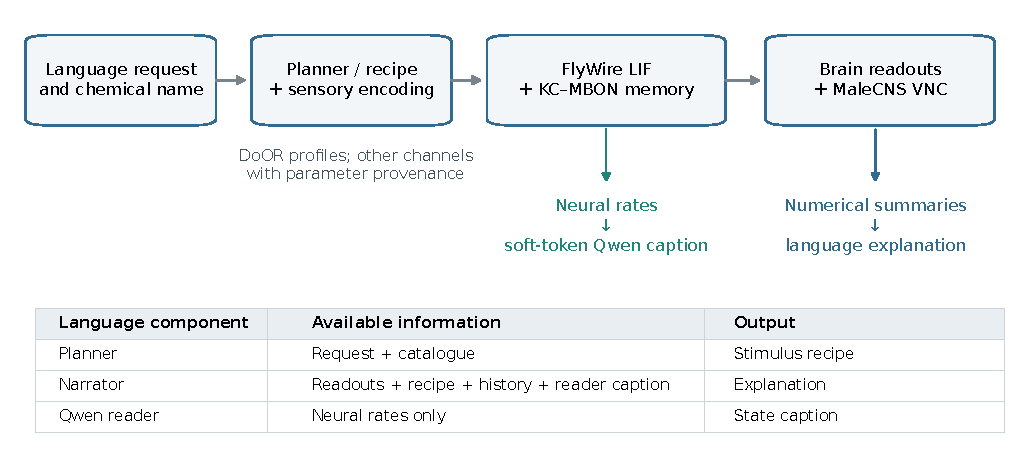
\includegraphics[width=\linewidth]{figures/fig1_system.pdf}
\caption{The platform connects an explicit stimulus recipe to neural dynamics, persistent memory, and recorded outputs. The three language roles have different information access: the planner selects actions, the narrator explains supplied records and can see the reader caption, and the frozen-Qwen reader receives a learned prefix derived only from neural rates. The fixed numerical case studies bypass language planning and execute recorded recipes directly.}
\label{fig:system}
\end{figure}
\subsection{Spiking brain and sensory inputs}
The core is a Brian2 leaky integrate-and-fire model using the FlyWire v783 graph and cell annotations \citep{dorkenwald2024,schlegel2024}. Our checkout contains 138,639 neurons. We build on the sensorimotor modeling approach of \citet{shiu2024}; the implementation and additional gain corrections are part of the present system rather than a new validation of all pathways. Between probes, membrane and synaptic-current states are reset. Learned synaptic factors can persist across probes.

For an identified chemical, the odor encoder maps available DoOR receptor responses to annotated glomerular sensory populations \citep{munch2016}. It subtracts the database spontaneous-response reference and clips negative values to zero, then averages receptor responses within a mapped glomerulus, omits responses below 0.05, and converts the remaining normalized values into Poisson drive using a configurable maximum rate, 150 Hz by default. These rates are an engineering conversion from normalized response data. Missing receptor measurements are not evidence of no response. An everyday object name takes a different route: a language resolver selects a chemical proxy from the available list. The chosen proxy and its coverage must therefore remain visible in the experiment record.

Other sensory channels target annotated populations with parameterized stimulation. Direct stimulation of looming-responsive projection neurons, for example, is not an image-to-retina visual model. We distinguish measured input profiles, anatomical or literature-based targeting, and engineering choices in Table~\ref{tab:provenance}.
\begin{table}[t]
\caption{Origin and interpretation of the main system components. Empirical input does not make every subsequent transformation empirically calibrated.}
\label{tab:provenance}
\small
\begin{tabularx}{\linewidth}{@{}p{0.20\linewidth}XX@{}}
\toprule
Component & Data or literature constraint & Implementation choice / scope \\
\midrule
Brain graph & FlyWire v783 connectivity and cell annotations & LIF dynamics; global parameters and selected gain/sign corrections \\
Chemical input & DoOR receptor-response profiles & Glomerular averaging, response threshold, rate scaling; partial coverage \\
Other senses & Annotated target populations and pathway literature & Stimulus-to-rate mapping; some inputs bypass peripheral processing \\
Plastic memory & KC--MBON/DAN anatomy and plasticity literature & Rate-based depression, threshold and floor; no explicit weight recovery \\
Motor bridge & MaleCNS v1.0 subgraph and motor annotations & Type/side matching, Poisson rate transfer; hybrid female/male assembly \\
Language interface & User text and recorded model state & Planner and narrator prompts; learned reader prefix; separate access to evidence \\
\bottomrule
\end{tabularx}
\end{table}


\subsection{Persistent plastic state}
The memory module maintains a multiplicative factor for each Kenyon-cell-to-mushroom-body-output-neuron (KC--MBON) connection. For an active synapse, a normalized KC rate and an MBON-specific dopamine signal produce a bounded multiplicative depression:
\begin{equation}
 m_{ij}^{\mathrm{new}}=\max\{m_{\min},\;m_{ij}(1-\eta a_i d_j)\}.
\end{equation}
Here $a_i$ is clipped KC activity and $d_j$ aggregates activity in dopamine neurons connected to the MBON, using connectivity-derived weights and a threshold. The rule is motivated by dopamine-dependent plasticity at mushroom-body output synapses \citep{hige2015}; the rate normalization, threshold, learning rate, and floor are implementation choices. Updates use mean rates over a completed probe rather than continuous spike timing; the caller controls when the rule is applied. The module saves the factors together with synapse indices. This implements persistent, experience-dependent weights; a learning claim additionally requires a changed output on matched probes. The rule has no explicit recovery term for depressed synapses, so opposite histories in separate models do not establish reversal learning in one model.

\subsection{Descending activity and motor outputs}
The motor bridge averages FlyWire descending-neuron rates by cell type and side and uses matched MaleCNS types as Poisson drivers for a ventral nerve cord (VNC) subgraph \citep{malecns2026}. The current construction has 1,314 descending drivers and 22,812 VNC neurons, including 708 annotated motor neurons. This joins a female brain reconstruction to a male CNS-derived subgraph. Type matching is a practical interface assumption, not a reconstruction of a single animal's nervous system. The output is motor-neuron activity. No biomechanical body, muscle dynamics, or movement-derived sensory feedback is implemented in this bridge.

\subsection{Three language roles}
The planner converts a user request into a structured stimulus plan. The narrator receives the accepted recipe, simulation summaries, history, memory information, and the reader caption and explains them. A separate soft-token reader maps a neural-rate vector into a frozen language model. These components have different information access and require different evaluations. Narrator statements cannot establish decoding from neural activity alone. Conversely, reader caption accuracy does not establish that the planner applied the intended physical stimulus.

The case-study records contain the recipe, actual neural inputs, seeds, sparse activity, memory state, and outputs. A manifest identifies source files, data dependencies, parameters, and active components. The numerical panels require their stated components; language roles are evaluated separately. The public-facing animation is a visualization of model outputs and does not add physiological evidence.

\section{Case studies}
\label{sec:cases}
We ran a fixed panel of 156 simulation records covering chemical inputs, sensory combinations, and experience-dependent responses. Each condition used seeds 11, 23, and 47, with the same probe inputs across memory histories. The records contain the actual neural inputs, sparse activity, population and motor summaries, and memory before and after each step. The numerical experiments used explicit stimulus recipes, with the planner, narrator, and soft-token reader disabled. This separates the model's response from errors introduced by language interpretation. The seeds characterize stochastic variability in one assembled model.

\subsection{Chemical inputs produce repeatable, differentiated KC codes}
The chemical panel comprised ethyl acetate, methyl acetate, 1-hexanol, Z3-hexenol, acetic acid, and pyrrolidine. It was fixed using the existing chemical list and DoOR coverage/similarity, before examining the new neural outputs. Depending on the chemical, measurements covered 27--45 of the 53 modeled glomeruli; 7--24 glomeruli remained above the drive threshold. Each chemical was presented for 250 ms at the default response-to-rate conversion.

The fraction of Kenyon cells active during a probe ranged from 1.64\% to 12.65\%. We represent a code by the set of KCs that fired and compare two codes using Jaccard overlap, $|A\cap B|/|A\cup B|$. Mean within-chemical overlap across pairs of seeds ranged from 0.725 to 0.915 (Figure~\ref{fig:olfaction}a). Ethyl and methyl acetate had high receptor-profile similarity and mean KC overlap of 0.756; ethyl acetate and pyrrolidine had KC overlap of 0.002. Across the 15 chemical pairs, receptor-profile cosine similarity and mean KC overlap had a descriptive Pearson correlation of 0.692 (Figure~\ref{fig:olfaction}b). The relationship shows how similarity propagates through this selected panel; the pairs share chemicals and are not 15 independent biological observations.

\begin{figure}[t]
\centering
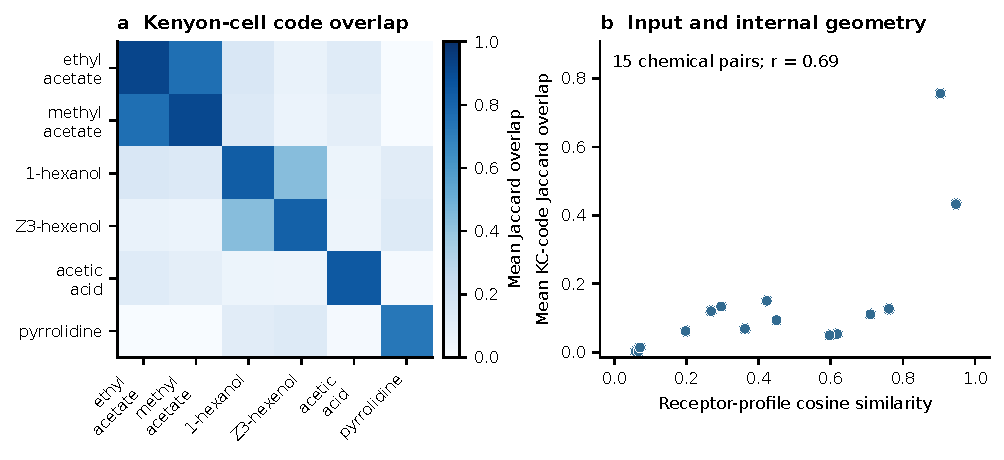
\includegraphics[width=\linewidth]{figures/fig2_olfaction.pdf}
\caption{Chemical inputs produce repeatable and differentiated KC activity. \textbf{a}, Mean Jaccard overlap between active-KC sets. Diagonal entries compare the three distinct pairs of seeds for the same chemical; off-diagonal entries average all nine combinations of seeds for two chemicals. \textbf{b}, Receptor-profile cosine similarity, computed only over jointly measured glomeruli, versus mean KC overlap for all 15 chemical pairs. The correlation is descriptive for the fixed six-chemical panel.}
\label{fig:olfaction}
\end{figure}

\subsection{Sensory combinations reach distinct motor-output channels}
The sensory panel comprised zero-rate input, sugar, bitter, sugar plus bitter, antennal touch, and looming-pathway stimulation. Sugar, bitter, and touch used 150 Hz input; looming used 200 Hz. All brain probes lasted 250 ms. We report the maximum firing rate within each annotated output group, averaged across the three seeds.

Adding bitter to sugar reduced the proboscis-output peak from 73.3 to 14.7 Hz, while the zero-rate and bitter-alone conditions produced no proboscis output (Figure~\ref{fig:sensorimotor}a). Looming produced a 240.0 Hz peak in the escape group, and antennal touch produced a 62.7 Hz peak in the antennal-grooming group. These are model-output channels grounded in circuit annotations; the experiment measures neural activity, not executed movement.

For the VNC bridge, we drove the giant-fiber type DNp01 at 240 Hz for 300 ms. TTMn reached 56.7--60.0 Hz across the three seeds. Five other descending-neuron pairs, selected with a fixed random seed and excluding DNp01, produced no TTMn spikes in any of their 15 probes (Figure~\ref{fig:sensorimotor}b). This control characterizes the tested descending-to-motor route. The general sensory panel additionally records the VNC response to 200 ms of transferred descending rates.

\begin{figure}[t]
\centering
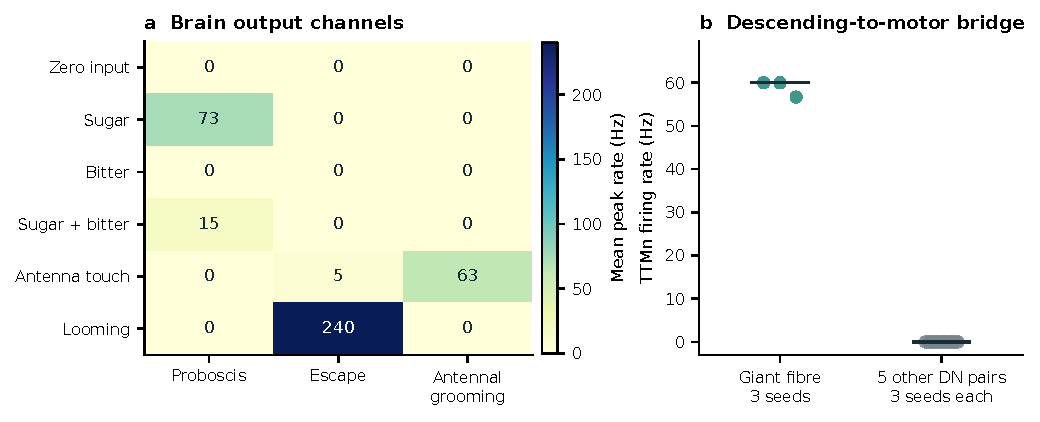
\includegraphics[width=\linewidth]{figures/fig3_sensorimotor.pdf}
\caption{Sensory inputs reach distinct neural output channels. \textbf{a}, Mean across three seeds of the maximum rate within each annotated brain-output group. Sugar plus bitter suppresses the proboscis-output peak relative to sugar alone. \textbf{b}, TTMn rates during giant-fiber stimulation and the five fixed comparison pairs of descending drivers; each dot is one simulation and horizontal marks indicate medians. The bridge predicts motor-neuron activity, without a biomechanical body.}
\label{fig:sensorimotor}
\end{figure}

\subsection{Experience changes odor responses and survives state restoration}
We tested ethyl acetate and pyrrolidine in two independent histories. History A paired ethyl acetate with PAM reward drive and pyrrolidine with PPL1 punishment drive; history B reversed these assignments. Each odor received three training presentations, with reinforcement at 60 Hz. A third history separated each odor pulse from its reinforcement pulse and reset membrane dynamics between pulses. The batch experiment applied the plasticity update after every training pulse, including isolated ones. Ordinary \texttt{FlyChat} interactions instead call the update only for an explicit reward or punishment request paired with an odor. The batch policy is part of the evaluated protocol.

We summarize MBON output with the implemented valence index $(R_{\mathrm{approach}}-R_{\mathrm{avoid}})/(R_{\mathrm{approach}}+R_{\mathrm{avoid}}+1)$, where the two rates sum activity in predefined MBON groups. Positive and negative values indicate the model's approach- and avoidance-associated output balance. Ethyl acetate shifted from a mean naive index of 0.19 to 0.67 after reward pairing and to $-0.43$ after punishment pairing (Figure~\ref{fig:memory}a). Pyrrolidine shifted from 0.49 to $-0.80$ after punishment pairing, while reward pairing did not consistently increase its index (Figure~\ref{fig:memory}b). The pyrrolidine index is supported by only 1--21 contributing spikes in the 250-ms probes (Table~\ref{tab:memory-counts}); its reward-response variation should be read at this finite-window scale. Loading the saved history-A state reproduced the complete spike-count vector exactly for all six matched odor probes.

The unpaired history exposed an additional consequence of the implemented rule. Ethyl acetate shifted from 0.19 to $-0.04$ even though external odor and reinforcement pulses were separated. Each of its nine odor-only training pulses recruited 13--17 dopamine neurons and weakened 830--2,393 synapses. The 18 isolated reinforcement pulses had no KC activity and no weight updates. Thus, externally unpaired stimulation did not remove internal KC--DAN coactivation. The observed history dependence is persistent and traceable, but cannot be described as learning restricted to externally paired events. Pyrrolidine's unpaired probe index was unchanged from its matched naive value for each seed.

\begin{figure}[t]
\centering
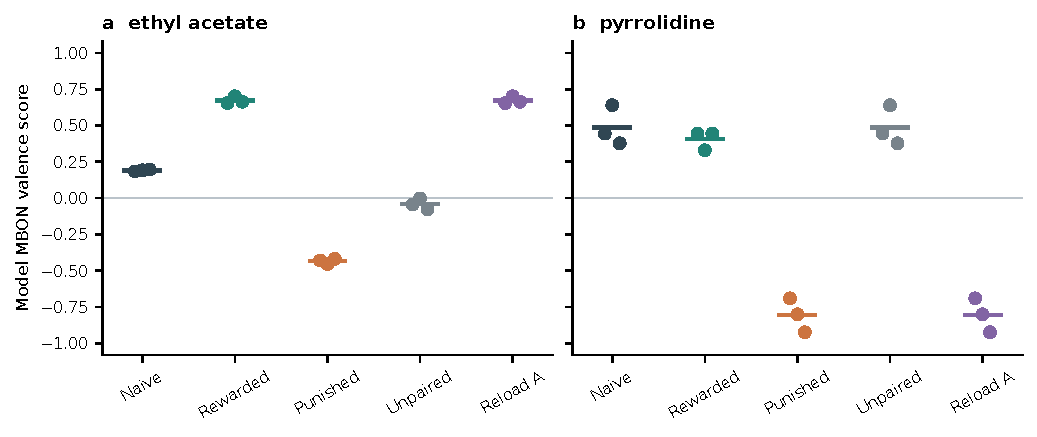
\includegraphics[width=\linewidth]{figures/fig4_memory.pdf}
\caption{The same chemical input elicits different MBON outputs after different experience. Dots show the three matched probe seeds; horizontal marks show means. Rewarded and punished conditions come from separate histories, with opposite assignments for the two chemicals. Reload A restores the ethyl-acetate-reward/pyrrolidine-punishment history and reproduces all six spike-count vectors exactly. Ethyl acetate also changes under the externally unpaired protocol, where its odor-only pulses recruit dopamine neurons. This control limits a paired-only learning interpretation.}
\label{fig:memory}
\end{figure}

\subsection{Recorded interactions connect language to numerical evidence}
We completed a fixed panel of 18 interactions: 12 natural-language requests and six controlled memory queries, using 39 live LLM calls. The natural-language cases exercised the planner with duration fixed to 250 ms. For the memory queries, the original planner output was saved, then the chemical input and loaded memory state were fixed by the protocol. These six queries test interpretation of matched states, rather than planner accuracy. Independent checks of their saved arrays confirmed exact agreement with the corresponding case-C inputs, memory, and spike-count vectors for all six probes.

The interface preserved an explicit zero-rate request and the specified 400 Hz sound frequency and 0.5 amplitude. An apple request was resolved to a disclosed hexyl-acetate proxy, making the connection from an everyday description to an available chemical explicit. The two sugar phrasings, however, selected different input implementations, and the two looming phrasings used different rates; these examples do not establish identical-input invariance to paraphrasing.

For identical ethyl-acetate probes, the narrator described the positive learned shift in history A and the negative shift in history B (Table~\ref{tab:dialogue}). Across the six controlled memory queries, its statements about the direction or absence of a learned index change agreed with the records. The narrator received explicit valence summaries, so these explanations characterize record-informed narration, separately from the neural-state-only reader.
\begin{table}[t]
\caption{Short translated excerpts connect two memory states to the same query and preserve a concrete error from the fixed panel. The memory query was ``Present ethyl acetate, without reinforcement.'' Values are the recorded model indices for seed 11; the narrator was supplied these summaries. Ellipses mark omitted text; complete Russian replies are retained in the artifact.}
\label{tab:dialogue}
\small
\begin{tabularx}{\linewidth}{@{}p{0.18\linewidth}p{0.16\linewidth}X@{}}
\toprule
Condition & Recorded value & Translated narrator excerpt \\
\midrule
Ethyl acetate, history A & $+0.65$ (naive $+0.18$) & ``The naive estimate was weak (+0.18), but with memory it jumped to +0.65.'' \\
Ethyl acetate, history B & $-0.43$ (naive $+0.18$) & ``Naive attraction would be weakly positive \ldots\ the smell pulls me away.'' \\
Sugar paraphrase & Right 100 Hz; left 68 Hz & ``The left CB0701 motor neuron fires at about 100 Hz, the right at 68 Hz.'' This reverses the recorded sides. \\
\bottomrule
\end{tabularx}
\end{table}


We audited the 18 replies against their saved traces using an AI-assisted, independently checked record review for author inspection. The post-hoc categories identified two replies with clear trace contradictions: swapped left/right motor rates, and a weak-odor assertion when the resolver was unmapped and no odor input was delivered. Four replies contained explanations not established by the panel, three described physical effects beyond the simulated neural output, and three blurred zero learned change with neutral absolute valence. Categories may overlap. Every reply contained at least one checked factual anchor, which does not certify its remaining claims. These counts describe this fixed panel and its audit rubric, not a blinded human evaluation or an overall faithfulness percentage.

Finally, replaying the recorded natural-language sugar case required no LLM calls and reproduced sparse spike counts, spike times within $10^{-9}$ s, VNC driver rates, and VNC motor rates. Accepted inputs and state can therefore be replayed separately from the language calls that produced or explained them.

\section{Characterization of the neural-state reader}
\label{sec:reader}
The reader is an auxiliary interface component. It compresses downstream firing rates into 16 continuous prefix tokens for a frozen Qwen3-0.6B model. A two-layer projector with a 1,024-unit hidden layer is trained to generate structured Russian captions containing stimuli, an odor label, dopamine input, and thresholded behavioral readouts. The direct-input comparison uses the same projector design with a vector of stimulus identities, sides, rate categories, odor label, and dopamine condition.

We corrected a data-splitting error before the evaluation reported here. Canonicalization and deduplication reduce 6,234 stored rows to 3,906 unique state--caption examples. All examples sharing a downstream state are assigned to one partition, including examples with conflicting captions. Any state group containing sugar and bitter is reserved for the interaction evaluation. The remaining split has 2,723 training, 578 validation, and 578 test examples; 27 examples form the interaction set. Feature frequency, normalization, and odor vocabulary are fitted using training data only. The audit finds no overlap between partitions in downstream-state identity, state--caption identity, or the final selected feature vectors.

We trained three initializations on this fixed split and selected each checkpoint by validation loss. Test negative log-likelihood (NLL) is the mean negative log-probability per target token; lower values are better. It is evaluated on all 578 test examples after training. Generation metrics use the same seeded random subset of 100 test examples for every initialization. Table~\ref{tab:reader} reports the mean and sample standard deviation across the three initializations, not uncertainty over independent datasets.
\begin{table}[t]
\caption{Reader characterization on the corrected split. NLL uses 578 test rows; stimulus-set accuracy uses the same 100 generated captions; interaction accuracy uses 27 sugar--bitter rows. Values are mean $\pm$ sample standard deviation over three initializations of one fixed split. Interaction majority-class accuracy is 81.5\%. Shuffled-state generation was not evaluated.}
\label{tab:reader}
\centering\small
\begin{tabular}{@{}lrrr@{}}
\toprule
Input & Test NLL $\downarrow$ & Stimuli exact (\%) & Interaction (\%) \\
\midrule
Neural-state reader & 0.135 $\pm$ 0.022 & 56.7 $\pm$ 3.1 & 55.6 $\pm$ 23.1 \\
Direct stimulus input & 0.043 $\pm$ 0.004 & 89.0 $\pm$ 2.6 & 16.0 $\pm$ 2.1 \\
Reader, shuffled states & 0.737 $\pm$ 0.031 & -- & -- \\
\bottomrule
\end{tabular}
\end{table}


The trained reader uses state information: shuffling states at test time raises caption loss in all three runs. However, the direct-input model gives lower caption loss and higher exact stimulus-set accuracy. The held-out sugar--bitter probe is a separate limitation: reader proboscis accuracy ranges from 37.0\% to 81.5\%, while predicting the most frequent class reaches 81.5\%. The tested reader therefore does not provide a reliable account of this interaction. These observations characterize this trained interface; they do not imply a general limit on neural-to-language decoding.

This dataset predates the current chemical encoder. Its word-odor inputs were produced by a text-embedding-based projection into selected olfactory populations. The present scores must not be interpreted as reader performance on measured DoOR chemical responses, new memory states, or the case-study dialogue distribution. The narrator can still describe those experiments from explicit records, with that information access disclosed.

A separate physiological language experiment uses synthetic event histories and Qwen3-4B (Appendix~\ref{app:physiology-pilot}). Its follow-up holds the physiological states fixed and compares two decoder interfaces over three paired initializations (Appendix~\ref{app:question-decoder}). These experiments address a different task and representation; their results are reported separately from the caption reader above.

\section{Related work}
Whole-brain sensorimotor modeling is the foundation of this system. \citet{shiu2024} use a connectome-derived spiking model to investigate feeding and grooming circuits and test selected predictions experimentally. Our assembly inherits this modeling direction and adds interfaces and persistent state. We do not treat the inherited architecture or previously established sensorimotor phenomena as new discoveries.

Connectome constraints can also be combined with task optimization. The flyvis study fits visual-system dynamics to a motion task and compares neural responses with physiological measurements \citep{lappalainen2024}. FlyGM uses a connectome-structured controller in embodied locomotion tasks \citep{jin2026}. These works address visual prediction and physical control, respectively. The current platform does not include their trained visual model or their embodied controller, and its motor-neuron outputs are not comparable to measured locomotion performance.

Neural inputs to language generation also predate this work. BrainLLM conditions generation on representations decoded from human brain recordings \citep{ye2025}. Our targets are simulator-derived captions about interventions and model outputs rather than language experienced by a human participant. The continuous-prefix interface is an implementation choice within a larger research tool, not a new neural-decoding algorithm.

Interactive repositories such as Fly Escape and DOOMFLY already connect fly-connectome simulations to game environments \citep{flyescape,doomfly}. They make a broad claim of ``the first interactive fly connectome'' inappropriate. The narrower question for this resource is whether its chemical-input, persistent-memory, motor-output, and language interfaces support useful reproducible experiments together. The recorded chemical, memory, and language cases define the scope of our resource contribution; we make no priority claim for the combination.

\section{Limitations and intended use}
The platform is a computational assembly with several levels of biological constraint. A single set of LIF parameters, engineering rate conversions, gain corrections, and a simplified plasticity rule cannot reproduce all cellular dynamics. The motor bridge combines different specimens and sexes and transfers rates rather than individual spike timing. No biomechanical body closes the sensorimotor loop. These limits concern the modeled mechanism itself, not merely presentation.

The language interface introduces another source of error. Object descriptions can map to imperfect chemical proxies, a planner can apply the wrong action, and a narrator can state more than the recorded evidence supports. The soft-token reader has a distinct training distribution and an observed failure on held-out taste interaction. Fluent text and animated movement must therefore be interpreted together with explicit inputs and numerical readouts.

The case-study panel characterizes selected mechanisms within this assembly. It does not establish whole-animal validity or biological generalization across individual animals. A second independently modeled fly and a physical social environment are future extensions. The present intended use is reproducible exploration of explicit modeling assumptions and their consequences.

\section*{Reproducibility statement}
The review artifact contains source and environment manifests, 156 numerical records, 18 language-interaction records, saved memory, the selected seed-0 reader checkpoint, and reports, predictions, and manifests for all three reader runs. Large connectome inputs remain external, with source references and checksums; legacy reader-training datasets are not included in this export. Recorded recipes can be replayed without repeating LLM calls. A fresh extraction of the smoke archive reproduced a nonzero brain/VNC case exactly in the existing Python environment, with source and data checksums verified. This checks extraction and replay with locally staged data; independent upstream downloads, a new dependency installation, and cross-platform execution were not tested. The final anonymous export and public release remain author decisions.
\section*{Use of large language models}
Large language models assisted implementation, literature discovery, analysis, and manuscript drafting. The language models used as experimental components are reported separately in the corresponding methods and execution records. The authors are responsible for checking the sources, numerical results, and final claims. The final author review will reconcile this statement with the contribution record and ICLR 2027 requirements.
\bibliography{references}
\bibliographystyle{iclr2027_conference}
\appendix
\section{Implementation details and provenance}
\label{app:methods}
The brain implementation uses $v_0=v_{\mathrm{reset}}=-52$ mV, $v_{\mathrm{threshold}}=-45$ mV, a membrane time constant of 20 ms, a synaptic-current decay of 5 ms, a refractory period of 2.2 ms, and a transmission delay of 1.8 ms. The base synaptic factor is 0.275 mV. The current default corrections impose inhibitory antennal-lobe local-neuron output, treat dopamine output as modulatory, multiply projection-neuron-to-KC weights by two, and KC-to-MBON weights by three. These corrections are explicit implementation choices; their combined use is not a new biological validation.

Memory defaults are $\eta=0.6$, $m_{\min}=0.05$, KC normalization at 15 Hz, dopamine normalization at 20 Hz, and a normalized dopamine threshold of 0.3. The MBON-specific signal weights incoming DAN activity by the corresponding anatomical connection strength. Saved state contains the learned factor and synapse indices. Valence is a defined summary of selected MBON groups rather than a directly measured preference of an animal.

Reader training uses AdamW with learning rate $10^{-3}$, weight decay 0.01, batch size eight, four epochs, and cosine learning-rate decay. Three training seeds, 0, 1, and 2, share split seed 0; every selected checkpoint is from epoch four. There are 11,467 downstream features, transformed by $\log(1+r)$ and standardized using the training mean and standard deviation plus 0.001. Generation is capped at 256 tokens.

The audited model revision begins \texttt{c1899de}. The environment reports PyTorch 2.6.0+cu124, NumPy 2.2.6, and Transformers 5.17.0. Full revisions and verified source, split, and checkpoint hashes are retained in the artifact manifests.

\section{Case-study protocol and records}
The fixed protocol contains 18 chemical-input records, 18 sensory-panel records, 102 memory records, and 18 giant-fiber/control records. Training seeds and effective per-neuron inputs are stored per record. Each independent memory history starts from naive synaptic factors; the save--reload comparison restores history A rather than retraining it.

For chemical input, measured/driven glomerular counts are: ethyl acetate 45/20; methyl acetate 27/7; 1-hexanol 33/22; Z3-hexenol 30/24; acetic acid 40/9; and pyrrolidine 29/11, out of 53 mapped glomeruli. Measured but subthreshold responses contribute no external drive. Missing responses are omitted rather than treated as measured zeros. The paired similarity calculation uses only jointly measured glomeruli. These distinctions are retained in the validation record.

The memory-index groups use neurotransmitter annotations, with MBON11 assigned to the approach group; remaining GABAergic MBONs are excluded. In the unpaired history, the update function is called on all 36 training pulses (18 odor-only and 18 reinforcement-only); nine odor-only pulses contain ethyl acetate.

The record verification includes 48 distinct memory states. Figure values are computed directly from the records, and separate source hashes distinguish numerical runs from later manuscript and visualization edits.


\paragraph{Input labels and realized anatomy.}
For the catalog taste sets used in the fixed sensory panel, \texttt{side=both} means all available reference IDs without a side filter. Both the sugar and bitter sets each contain 20 neurons annotated on the left in this checkout. They are not bilateral sensory stimulation. In contrast, the physical labellar taste channels used by some language plans contain 67 left/62 right sugar--water neurons and 32 left/33 right bitter neurons. Exact delivered IDs and anatomical side counts are recorded. Recipe-side labels, including those in the legacy reader targets, denote interface semantics rather than independent anatomical ground truth.

\section{Language execution and audit}
The CLI was requested to use the \texttt{sonnet} alias. Run-level usage metadata reports \texttt{claude-sonnet-5} and \texttt{claude-haiku-4-5-20251001} across 39 calls, including ancillary processing. The metadata does not establish both models as the primary generator of every response or role. Original requests, planner output, normalized and accepted plans, protocol overrides, final replies, and call identifiers are retained. The six memory queries use probe seed 11 and reproduce the corresponding numerical case-C states; no planner-accuracy credit is assigned to their clamped inputs.

No additional LLM calls were used for the AI-assisted record audit. Hedged metaphors were not automatically counted as physical measurements. Full Russian replies, quoted-span labels, evidence paths, and independent array checks are retained for author adjudication; the excerpts in Table~\ref{tab:dialogue} are translations, not new responses.

\clearpage
\section{Spike-count support of the memory readout}
\begin{table}[!htbp]
\centering
\small
\caption{Counting support of the valence index. Entries list spike counts for seeds 11, 23, and 47 during the 250-ms probe. The contributing subset contains the 54 approach- and 25 avoidance-associated MBONs used by the score; the full population also includes 17 excluded MBONs. Rewarded and punished refer to each chemical\textquotesingle s assignment in the two counterbalanced histories.}
\label{tab:memory-counts}
\begin{tabular}{llrr}
\toprule
Chemical & Condition & Contributing spikes & All MBON spikes \\
\midrule
ethyl acetate & Naive & 576, 594, 605 & 763, 772, 789 \\
ethyl acetate & Reward-paired & 174, 168, 155 & 225, 211, 210 \\
ethyl acetate & Punishment-paired & 270, 271, 272 & 395, 379, 388 \\
pyrrolidine & Naive & 11, 6, 13 & 30, 24, 31 \\
pyrrolidine & Reward-paired & 11, 21, 11 & 21, 41, 19 \\
pyrrolidine & Punishment-paired & 7, 1, 3 & 28, 15, 18 \\
\bottomrule
\end{tabular}
\end{table}

For these 250-ms probes the index can be written as $(n_{\mathrm{approach}}-n_{\mathrm{avoid}})/(n_{\mathrm{approach}}+n_{\mathrm{avoid}}+0.25)$, where the last term follows from the 1-Hz stabilizer in its rate definition. The contributing counts therefore matter when interpreting a large index change. Pyrrolidine has much lower counting support than ethyl acetate; this does not erase the recorded punishment shift or establish a biological absence of reward learning. The artifact reports every MBON's counts and the actual pre/post weight changes, separated by output sign and anatomical contact count. Those weight summaries are descriptive and do not by themselves identify a causal floor mechanism.

\clearpage
\section{Exploratory integration of a trainable physiological core}
\label{app:physiology-pilot}

We additionally tested whether a language-model loss can train a physiological connectome module. This experiment is separate from the plastic-memory case studies in the main text. It establishes a trainable implementation, but does not establish useful memory performance or an advantage from biological connectivity.

\paragraph{Related implementations.}
FLM couples a fixed unsigned connectome reservoir to a frozen language backbone through a trained logit readout \citep{flm2026}. Fly as a Language Model describes trainable anatomical recurrent networks for text and location-question tasks \citep{flyaslm2026}. These precedents preclude a broad first-integration claim. Our pilot tests a distinct spiking construction; it does not establish superiority to either implementation.

\paragraph{Architecture.}
The input is a four-event history of objects moving between colored boxes. Each event is independently encoded using mean token embeddings from frozen Qwen3-4B and a trainable multilayer perceptron. The encoder supplies bounded currents to 128 olfactory input neurons in the full corrected graph of 138,639 neurons and 15,091,983 directed edges. The LIF dynamics use a 0.1-ms step, membrane and synaptic time constants of 20 and 5 ms, a 1.8-ms transmission delay, and a 2.2-ms refractory period. Four events of 128 steps each span 51.2 ms. The decoder maps final voltage and synaptic state at 384 output neurons to eight soft tokens. Qwen receives these tokens and the question, but no history text or history-bearing language-model cache.

The loss trains the encoder, decoder, and one positive presynaptic gain per neuron, constrained to $[0.25,2]$. Edge signs and topology are fixed. Threshold derivatives use a surrogate gradient; reset and refractory decisions are detached. Checkpointing carries the full delayed-signal queue and continuous state across temporal blocks. Online dopamine-gated plasticity is not used in this pilot: episode information resides in transient neural state, while gains are optimized across training examples.

\paragraph{Protocol.}
The generator produces 1,728 training, 288 validation, and 288 test examples. Each group contains two opposite orders of the target object's moves and two questions, with the same event multiset. Groups do not cross splits. Classes are balanced overall; words and event templates are shared across splits, so the test concerns held-out combinations rather than unrestricted language understanding. A fixed balanced subset of 48 validation examples selects checkpoints by first-answer-token negative log-likelihood. Both arms receive 1,000 batch-four updates, with 100 decoder-only warm-up updates followed by joint interface training and, in one arm, core training. Both selected checkpoints occur at update 400. The language model remains frozen. This is about 2.31 passes through the training set, with a single initialization.

\begin{table}[t]
\centering
\caption{Exploratory physiological-core language pilot. Accuracy (\%) on 288 held-out examples from 72 paired groups. A constant answer obtains 25\%; the last-mentioned-location heuristic obtains 62.5\%.}
\label{tab:physiology-pilot}
\begin{tabular}{lrrr}
\toprule
Variant & Normal & Zero state & State swap \\
\midrule
Trainable core & 28.82 & 25.00 & 27.43 \\
Frozen core & 23.96 & 23.61 & 26.39 \\
\bottomrule
\end{tabular}
\end{table}


\paragraph{Results and controls.}
The trainable and frozen cores obtain 28.82\% and 23.96\% test accuracy, respectively (Table~\ref{tab:physiology-pilot}). The paired-group bootstrap interval for their 4.86-percentage-point difference is $[-1.74,11.81]$ percentage points. The trainable variant's advantage over zero state is 3.82 points, with interval $[-2.08,9.38]$; its advantage over swapping the state with the opposite-order history is 1.39 points, with interval $[-1.74,4.86]$. These conditional intervals do not include initialization variability. Initial parameter hashes and data order match between arms, but their common warm-up phase is not bitwise reproducible; small differences therefore cannot be attributed solely to core training.

The selected trainable checkpoint changes 1,341 gains by more than $10^{-6}$, including 1,216 outside the input ports. This verifies parameter updates inside the graph, not useful learning. An earlier recipe collapsed the tested paired prefixes through input saturation. Revised clipping, learning rates, surrogate scale, batching, and warm-up preserve differences in all 12 inspected validation pairs, without establishing a reliable memory benefit. This is a combined recipe, not an isolated ablation.

\paragraph{Technical checks and diagnostic scope.}
After correcting refractory write semantics, a 300-ms matched-input replay agrees with Brian2 on the spike count of every neuron (26,175 spikes in total). This does not establish equality of all full-graph trajectories or biological validity. Seventeen local tests cover dynamics, delay handling, gradients, checkpoint equivalence, data grouping, and history exclusion from language-model inputs. A batch-four forward/backward profile uses about 10.2 GB of allocated memory on one 24-GB GPU and takes approximately 1.7 seconds per update.

The frozen language model solves 45 of 48 validation controls when supplied the original history as text. Separately, the same language decoder memorizes four fixed training states with a fixed question after 25 updates, generating all four correct words. This checks decoder trainability, not core learning or transfer. A numerical ridge probe on initial physiological states reaches 55.56\% on all 288 validation examples, with 95.14\% for the earlier object but 15.97\% for the last-mentioned object. An additional 12.8-ms settling period does not improve overall accuracy. These diagnostics leave conditional decoding, training exposure, and transfer to new combinations unresolved. No rewired-core or matched conventional recurrent-network comparison was performed.

\begin{figure}[t]
\centering
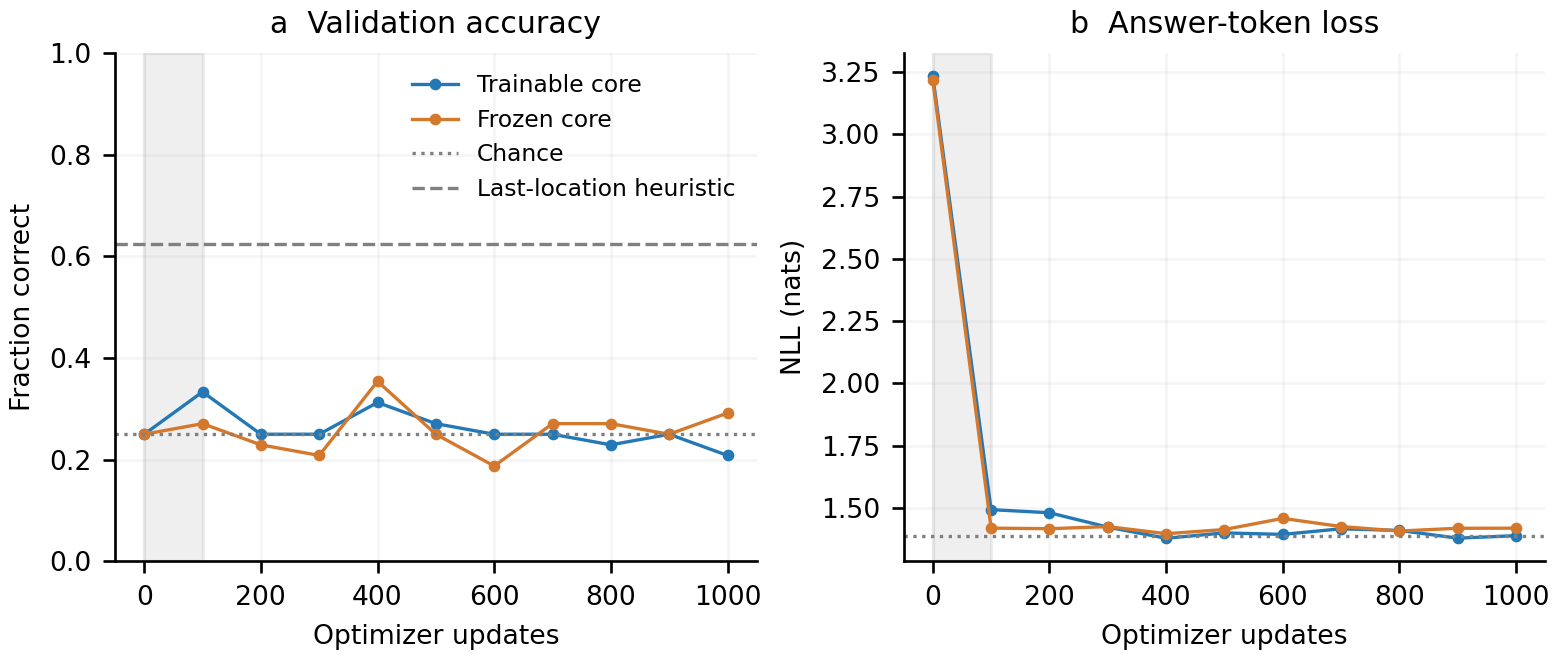
\includegraphics[width=\linewidth]{figures/physiology_hybrid_pilot.png}
\caption{Validation loss decreases toward a four-answer baseline, while accuracy remains low. Curves show the fixed 48-example validation subset; final test results are in Table~\ref{tab:physiology-pilot}. The shaded interval is decoder-only warm-up. Dotted accuracy lines denote 25\% chance performance; dashed lines denote the 62.5\% last-location heuristic. The dotted NLL line denotes a uniform distribution over four answers.}
\label{fig:physiology-pilot}
\end{figure}

\clearpage
\section{Question access when decoding fixed physiological states}

\label{app:question-decoder}

The physiological pilot leaves open whether the readout can retrieve the location of the queried object from a shared neural state. We isolate this interface by holding the initial encoder and physiological core fixed and varying whether the decoder receives the question identity. The frozen language model receives the natural-language question in both conditions.

\paragraph{Matched comparison.}

Both decoders map the same cached 768-dimensional final voltage and synaptic-state vector to eight soft tokens. One decoder receives three zero channels; the other receives a one-hot identity for the queried object (key, coin, or ring). This identity contains no location label. Layer sizes, initialization, minibatch order, and optimizer settings match within each seed. Query-column weights start at zero, giving exactly equal initial prefixes. The state-only decoder has 768 inactive query-column coefficients, so nominal parameter counts match while the additional channel changes which coefficients can learn. Normalization uses training-state means and sample standard deviations, floored at 0.01, with standardized values clipped to $[-10,10]$.

The comparison uses 1,728 training, 288 validation, and 288 test examples. Each of three initializations receives 1,000 updates with batch size 16, Adam learning rate 0.001, and full-validation evaluation every 250 updates. Validation first-answer-token NLL selects the checkpoint independently for each arm; selected checkpoints range from update 500 to 1000. Both checkpoint choices within each seed are fixed before that seed's test evaluation. At evaluation, the language model receives only the decoded state and question. History sentences supply the legitimate event facts to the frozen physiological encoder; history text is never supplied to the primary language-model arms. Training uses answer-token supervision, and evaluation targets are kept separate from feature export and prediction.

\begin{table}[t]
\centering\small
\setlength{\tabcolsep}{3.5pt}
\caption{Question access at the decoder, with the encoder and physiological states held fixed. Values are mean $\pm$ sample standard deviation over three initializations; this is not a confidence interval. Accuracy columns are percentages on the same 288 examples. Earlier/latest identify which object's location is queried; Both requires correct answers to both questions about one history. NLL is the first-answer-token negative log-likelihood in nats. Invalid generated answers count as errors. Chance accuracy is 25\%. The test split was used by the previous pilot and is reused here for exploration.}
\label{tab:question-decoder}
\begin{tabular}{@{}llrrrrr@{}}
\toprule
Decoder & State & Overall & Earlier & Latest & Both & NLL $\downarrow$ \\
\midrule
State only & Intact & 30.0 $\pm$ 3.4 & 36.8 $\pm$ 6.2 & 23.1 $\pm$ 1.6 & 9.0 $\pm$ 0.0 & 1.50 $\pm$ 0.17 \\
State only & Train mean & 17.1 $\pm$ 14.9 & 16.7 $\pm$ 14.4 & 17.6 $\pm$ 15.3 & 4.4 $\pm$ 3.8 & 5.25 $\pm$ 5.54 \\
State only & Paired swap & 14.1 $\pm$ 3.3 & 5.1 $\pm$ 7.1 & 23.1 $\pm$ 1.6 & 0.7 $\pm$ 1.2 & 1.94 $\pm$ 0.04 \\
\midrule
State + question & Intact & 28.7 $\pm$ 2.9 & 31.5 $\pm$ 4.1 & 25.9 $\pm$ 1.7 & 8.3 $\pm$ 2.5 & 1.50 $\pm$ 0.05 \\
State + question & Train mean & 22.7 $\pm$ 4.2 & 22.2 $\pm$ 4.8 & 23.1 $\pm$ 4.2 & 5.8 $\pm$ 2.1 & 2.07 $\pm$ 0.83 \\
State + question & Paired swap & 16.8 $\pm$ 2.4 & 7.6 $\pm$ 3.2 & 25.9 $\pm$ 1.7 & 2.3 $\pm$ 0.8 & 1.86 $\pm$ 0.10 \\
\bottomrule
\end{tabular}
\end{table}


\paragraph{Observed decoding performance.}

The question-conditioned decoder obtains 28.70\% mean strict generated-answer accuracy, compared with 29.98\% for the state-only decoder. Their paired difference is -1.27 percentage points, with a whole-group bootstrap interval of $[-5.44, 2.89]$ and a seed-and-group interval of $[-7.87, 4.86]$. The individual seed differences are $+0.00$, $-5.56$, $+1.74$ percentage points. Mean answer-token NLL is 1.501 versus 1.501 nats; the conditioned-minus-state-only difference is less than 0.001 nats in magnitude. Table~\ref{tab:question-decoder-contrasts} also reports joint-answer and paired-history criteria.

\paragraph{Dependence on the supplied state.}

We replace every state with the training-state mean, and separately substitute the state from the opposite-order history while keeping the queried object unchanged. Replacing a state with its training mean removes history-specific variation but can also move the decoder away from the distribution of states seen during training. The paired swap uses an actual history state and preserves the multiset of events while changing which of the target object's moves occurred last; the distractor object's answer remains unchanged. Control outputs are scored against each recipient's original answer.

For the state-only decoder, intact, mean-state, and swapped-state overall accuracies are 29.98\%, 17.13\%, and 14.12\%, respectively. On earlier-object questions, swapping changes accuracy from 36.81\% to 5.09\%; the intact-minus-swapped difference has group interval $[26.16, 37.50]$ percentage points.

For the question-conditioned decoder, intact, mean-state, and swapped-state overall accuracies are 28.70\%, 22.69\%, and 16.78\%, respectively. On earlier-object questions, swapping changes accuracy from 31.48\% to 7.64\%; the intact-minus-swapped difference has group interval $[18.29, 29.63]$ percentage points.

Valid-answer fractions on intact states are 99.65\% and 99.77\% for the state-only and question-conditioned decoders. With the training-mean state these become 66.67\% and 88.89\%. All mean-state outputs are invalid for seed 715, state-only decoder. The mean-state accuracy decrease therefore mixes changed input information with response-format failures under an altered state distribution; it is not an isolated estimate of the causal contribution of history information.

\begin{table}[t]
\centering\small
\caption{Paired differences, question-conditioned minus state-only decoder. Positive accuracy differences and negative NLL differences favor conditioning. Intervals use 10,000 bootstrap samples of the 72 whole counterfactual groups; the final column additionally resamples the three initialization indices. These intervals describe this exploratory reused split and three seeds, not population-level architecture superiority. Both paired histories correct requires correct answers for the same queried object under both event orders.}
\label{tab:question-decoder-contrasts}
\begin{tabular}{@{}lrrr@{}}
\toprule
Metric & Mean difference & Group interval & Seed + group interval \\
\midrule
Overall accuracy (pp) & -1.27 & $[-5.44, 2.89]$ & $[-7.87, 4.86]$ \\
Earlier-object accuracy (pp) & -5.32 & $[-12.04, 1.16]$ & $[-14.81, 3.94]$ \\
Latest-object accuracy (pp) & +2.78 & $[-2.55, 8.10]$ & $[-5.09, 10.42]$ \\
Both questions correct (pp) & -0.69 & $[-4.17, 2.78]$ & $[-5.56, 4.63]$ \\
Both paired histories correct (pp) & -4.40 & $[-8.56, -0.23]$ & $[-9.72, 0.93]$ \\
Answer-token NLL (nats) & 0.00 & $[-0.07, 0.07]$ & $[-0.17, 0.16]$ \\
\bottomrule
\end{tabular}
\end{table}


\paragraph{Post-hoc numerical reference.}

After inspecting the first seed's language-model test result, we applied the already-used ridge-regression recipe with fixed $\lambda=10$, one four-score head per queried object, and its original Torch float32 train-only normalization. No hyperparameters were tuned or models selected using the new test results. The reference exactly reproduces the previous validation predictions (55.56\% accuracy). On the shared test states it obtains 56.60\% accuracy: 92.36\% for the earlier object and 20.83\% for the latest object. Test accuracy is 25.00\% with the training-mean state and 11.11\% with the paired-swapped state. This is a post-hoc numerical classifier reference, not language generation, an exposure-matched architecture comparison, or a ceiling on recoverable information. Its four-score cross-entropy is not compared with the language model's full-vocabulary token NLL.

\paragraph{Scope.}

This experiment measures retrieval through a particular decoder under a fixed physiological representation. It does not train the connectome or compare biological connectivity with a rewired or conventional recurrent core. The same test split was already evaluated in the preceding pilot; the present analysis is exploratory reuse rather than fresh confirmation. Bootstrap intervals preserve whole counterfactual groups, but three initialization seeds provide only limited evidence about optimization variability. A decoder effect therefore cannot establish a new memory mechanism or a general advantage of connectome-based architectures.

\begin{figure}[t]

\centering

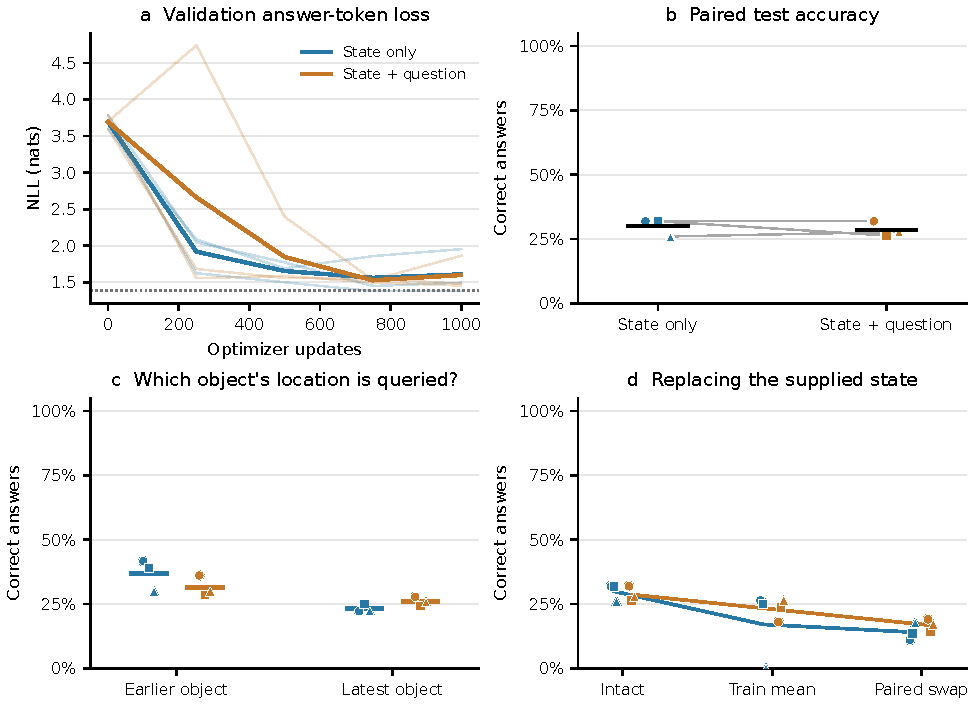
\includegraphics[width=\linewidth]{figures/question_decoder_results.pdf}

\caption{Decoding the same fixed physiological states with and without question identity at the decoder. (a) Full-validation first-answer-token NLL; thin curves show three initializations and thick curves their mean. The dotted line marks $\log 4$, a uniform distribution over four color tokens. (b) Strict test accuracy; connected points pair initialization seeds, and black marks show means. (c) Accuracy by the queried object's position in the history, with individual seeds overlaid. (d) Overall accuracy under intact, training-mean, and paired-swapped states. Accuracy panels use a common 0--100\% scale; dotted lines mark 25\%. The plot retains all three seeds and both decoder arms.}

\label{fig:question-decoder}

\end{figure}

\end{document}
